\documentclass[11pt]{amsart}
\usepackage{geometry}                % See geometry.pdf to learn the layout options. There are lots.
\geometry{letterpaper}                   % ... or a4paper or a5paper or ... 
%\geometry{landscape}                % Activate for for rotated page geometry
%\usepackage[parfill]{parskip}    % Activate to begin paragraphs with an empty line rather than an indent
\usepackage{graphicx}
\usepackage{amssymb,tikz}
\usepackage{epstopdf}
%\usepackage{multicolumn}
\usepackage{tabularx}
\usepackage{subcaption}
\usepackage{cite}
\DeclareGraphicsRule{.tif}{png}{.png}{`convert #1 `dirname #1`/`basename #1 .tif`.png}

\title{Methods}
\author{Nick Kappler}

\usepackage{hyperref}
\begin{document}
\maketitle
\section{Including Parasites (or, changing a few body size ratios)}


\subsection{Niche Models\label{sec:structure}}

We first generated 100 food webs with 40 species and connectance $C=0.15\pm .0075$ using the Niche Model.  The Niche model is an algorithm that generates realistic food webs with minimal inputs ~\cite{Williams2000}.\footnote{'We looked at alternatives but they did not pass muster.' Keep this in your back pocket.}  Figure \ref{fig:nicheModel} illustrates the model.  A species, $j$ is placed on the niche axis, $[0,1]$, by choosing a niche value uniformly randomly from $[0,1]$.  This species is then given a diet center and a diet width.  The diet width is calculated as $r_j=n_jy_j$.  In the calculation of diet width, $y_j$, is a random variable drawn from a beta distribution with $\alpha = 1$, and $\beta$ chosen so that the expected width of a diet is the desired connetance, $C$ ($\beta = (1-2C)/2C$).  The beta distribution is chosen so that the distribution of diet widths is approximately exponential, which means the distribution of generalities will be approximately exponential.  We multiply $y_j$ by $n_j$ so that species with higher niche values will tend to be more generalist than species with lower niche values.  A diet center, $c_j$, is chosen uniformly randomly such that $c_j \leq n_j$ and the diet falls entirely within the niche axis.  Species $j$ consumes a species $i$ if $n_i$ falls within the feeding range of $j$.  


\begin{figure}{h}
%This is a schematic of the Niche Model.
\begin{tikzpicture}
\draw (0,0)--(10,0)
node[anchor = west] {$n$};
\draw (0,.2)--(0,-.2)
node[anchor = north] {$0$};
\draw (10,.2)--(10,-.2)
node[anchor = north] {$1$};
%Predator
\fill (7,0) circle (.07) 
node[anchor = north]  {$n_j$};
%Predator Diet
\draw (7,0)--(7,.75)--(2,.75)--(2,.5);
\draw (.3,0) -- (.3,.5) -- (3.7,.5) -- (3.7,0);
\draw[dashed] (2,.5) -- (2,0) 
node[anchor = south east] {$c_j$};
\draw[<->] (.3,-.5) -- (3.7,-.5)
node[fill=white,pos = 0.5] {$r_j$}; 
\draw[dashed] (.3,0)--(.3,-.55);
\draw[dashed] (3.7,0)--(3.7,-.55);
%Prey
\fill (3,0) circle (.07) 
node[anchor = north west]  {$n_i$};
\draw(4.2,-2) circle (.3)
node {$i$};
\draw[->] (4.5,-2) -- (5.5,-2);
\draw(5.8,-2) circle (.3)
node {$j$};
\end{tikzpicture}
\caption{This figure demonstrates how feeding relationships are determined in the Niche Model.\label{fig:nicheModel}}
\end{figure}

\subsection{Allometric Trophic Network Model}

We simulated population dynamics on the food web structures described in section \ref{sec:structure} using the Allometric Trophic Network (ATN) model.  The ATN model is an easily parameterized and extensible model that is capable of reproducing realistic dynamics ~\cite{Boit2012}.  At the heart of the ATN model is the assumption that a species' metabolic rate controls both mortality and biomass accumulation (unless otherwise noted the choices that follow can be found in ~\cite{Brose2006}).  The dependence on this fundamental biological rate along with empirically supported allometric scaling laws means that the only species-specific parameter needed is body size.  We use the following formula to generate body sizes for any free-living species in a network structure:

\begin{equation}
M_i= Z_f^{TL_i-1}\label{eq:mFree}
\end{equation}

Where $TL_i$ is the prey-averaged trophic level of species $i$ and $Z_f$ is the average body size ratio of consumer $i$ to its prey ~\cite{Williams2004}.  $Z_f$ will therefore determine the average body size ratio of the entire food web.  This means that species at a given trophic level will be $Z_f$ times larger than species one trophic level lower.  However, this still allows for individual consumer-resource body size ratios to vary for each species since we use prey-averaged trophic level.  It is not possible to define body sizes such that all links have the same consumer-resource body size ratio.  We ran a full set of simulations for each of $Z_f = 10$ and $Z_f = 100$.  

Using the body size as defined in \eqref{eq:mFree}, we define the mass-specific metabolic rate as
\begin{equation}
x_i = a_{x_i} M_i^{-0.25}\label{eq:x}
\end{equation}
The $-0.25$ power has both empirical and theoretical support (~\cite{Brown2004}, others?).  The constant $a_{x_i}$ is the metabolic scaling constant that varies across metabolic classes of species.  In all simulations we take $a_{x_i}=0.314$, which is the value for a broad collection of invertebrate species.  With these fundamental constants in hand we can write the following dimensionless equations that govern the biomasses of all species in a food web (see ~\cite{Yodzis1992} for the original 2-species derivation and ~\cite{Williams2007} for an updated multi species derivation): 

\begin{subequations}\label{eq:atn0}
\begin{align}
\frac{dB_{b}}{dt} &= r_bB_b\left(1-\frac{\sum_{k\in\text{basal}}B_k}{K}\right) - \sum_kB_kx_k\frac{y_{bk}F_{bk}}{e_{bk}}\label{subeq:basal0} \\ 
\frac{dB_{c}}{dt} &= -x_cB_c + x_cB_c\sum_ky_{kc}F_{kc} - \sum_k x_kB_k\frac{y_{ck}F_{ck}}{e_{ck}} \label{subeq:con0}
\end{align}
\end{subequations}

Here $B_b$ and $B_c$ denote the biomass density of basal and consumer species, respectively; thus \eqref{subeq:basal0} and \eqref{subeq:con0} represent rates of change of basal and consumer populations, respectively (regardless of whether the consumer is a free-liver or parasite).  $r_b$ is the intrinsic growth rate of basal species $b$ and $K$ is the community carrying capacity of basal species.  $x_i$ is the mass specific metabolic rate of consumer $i$. $y_{ij}$ is the maximum assimilation rate of $i$ by $j$ relative to $j$'s metabolic rate that varies according to metabolic class of the consumer.  $e_{ij}$ is the assimilation efficiency of $j$ when consuming $i$ and varies according to the type of prey (autotroph or heterotroph prey item).  $F_{ij}$ is a normalized functional response of $j$ preying on $i$.  Note that this functional response represents how the \textit{assimilation} of biomass changes with changes in prey biomass, not the consumption of prey biomass.  It has the following form:
\begin{equation}
F_kj = \frac{\omega_{ij}B_j^{1+q}}{B_0^{1+h} + \sum_k\omega_{kj}B_k^{1+h}}\label{eq:fr0}
\end{equation}
Here $h$ quantifies deviation from a multi-species type II functional response, $\omega_{ij}$ is the relative preference for prey item $j$ by $i$, and $B_0$ is the half-saturation density.  When $h=0$ and $j$ has only one prey, $B_0$ is the density of prey that yields an attack rate on $i$ by $j$ equal to half the maximum attack rate; it is related to the handling time in more traditional formulations of type II functional responses.  In the case of multiple prey or $h\neq0$, $B_0$ is harder to interpret but generally affects how quickly the functional response approaches its saturating value.  

\subsection{Introducing Parasites\label{subsec:paraIntro}}

We controlled the number of parasites in our food webs by switching the roles of certain consumers from free-living species to parasitic species.  We chose which consumers to switch by first randomly ordering all consumers.  We then assigned the first fraction, $f_\text{par}$ of those species in the list to be parasites.  In this way, parasites at low levels of parasitism are also always parasites at higher levels of parasitism.  The same sequence of consumers was used for each simulation but each web necessarily had a different sequence.  This allowed for direct comparisons between models.  We used 11 different fractions of parasites evenly spaced from 0 up to 0.5, that is, from 0\% up to 50\% of consumers as parasites in increments of 5\%\footnote{We did not go past 50\% since interpreting parasites as parasites becomes difficult since their average consumer-resource body size ratio becomes close to the original value for free-living consumers}.

 In this study, the most basic difference between a free-living consumer and a parasitic consumer is the body size ratio of the parasite to its host species.  On average, a parasitic species will be much smaller than its host, whereas a free-living consumer will generally be much larger than its prey.  The body sizes of parasitic species were determined using the following formula (note that $k = \log Z_f$):

\begin{equation}
M_i = 10^{p + k(TL_i -2)} \label{eq:mPara}
\end{equation}

With this choice of body size, parasites will be on average $10^{p}$ times the size of their free-living hosts, $10^k$ times the size of their parasitic prey (same as free-livers on free-livers, the red dashed links in figure \ref{fig:bsrCartoon}), and $10^{p-2k}$ times the size of their free-living predators (the green dashed link in \ref{fig:bsrCartoon}.  The last ratio ($10^{p-2k}$) is not ideal since it significanty increases the average body size ratio of free-living consumers\footnote{Need to look at these plots}.  From the parasitic body sizes we derive the parasitic mass-specific metabolic rate using equation \eqref{eq:x}.  We a ran a full set of simulations with each of $p=-3$ and $p=-4$.  A schematic of the body size hierarchy defined by equations \eqref{eq:mPara} and \eqref{eq:mFree} is given in figure \ref{fig:bsrCartoon}.

\begin{figure}
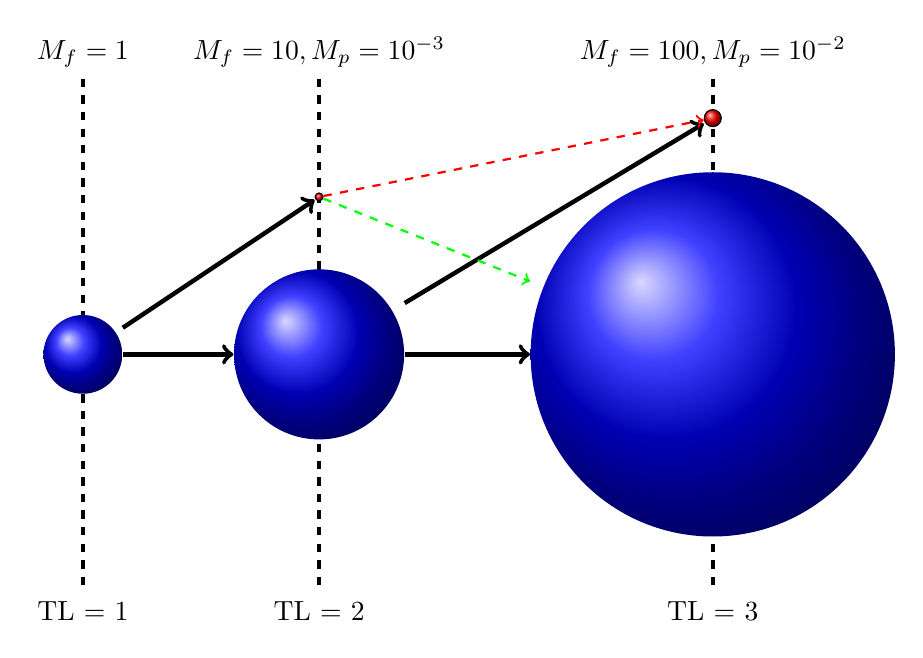
\begin{tikzpicture}
\node [inner sep = .05cm] (p1) at (3,1) {};
\node [inner sep = .108cm] (p2) at (8,2) {};
\node [inner sep = .5cm] (s1) at (0,-1) {};
\node [inner sep = 1.08cm] (s2) at (3,-1) {};
\node [inner sep = 2.313cm] (s3) at (8,-1) {};
\draw[->,ultra thick] (s1) -> (s2);
\draw[->,ultra thick] (s2) -> (s3);
\draw [ultra thick, dashed] (8,2.5) node [anchor = south]  {$M_f = 100,M_p=10^{-2}$}--(8,-4) node [anchor = north] {TL = 3};
\draw [ultra thick, dashed] (3,2.5) node [anchor = south]  {$M_f = 10,M_p=10^{-3}$}--(3,-4) node [anchor = north] {TL = 2};
\draw [ultra thick, dashed] (0,2.5) node [anchor = south]  {$M_f = 1$}--(0,-4) node [anchor = north] {TL = 1};
\draw[->,ultra thick] (s1) -> (p1);
\draw[->,ultra thick] (s2) -> (p2);
\draw[->,dashed,thick,red] (p1) -> (p2);
\draw[->,dashed,thick,green] (p1) -> (s3);
\shade [ball color=blue] (s1) circle (.5cm);
\shade [ball color=blue] (s2) circle (1.08cm);
\shade [ball color=blue] (s3) circle (2.313cm);
\draw [ball color=red] (p1) circle (.05cm);
\draw [ball color = red] (p2) circle (.108cm);
\end{tikzpicture}
\caption{This figure shows the body size hierarchy when body sizes are defined according to equations \eqref{eq:mPara} and \eqref{eq:mFree}. In this figure, the volume of the spheres scale logarithmically with the body size, and arrows denote biomass flow.  The situation in the model is also more complicated since we do allow fractional trophic levels.\label{fig:bsrCartoon}}
\end{figure}

\subsection{Models\label{subsec:models}}

As described in section \ref{subsec:paraIntro}, each web will be tested with different average body size ratios: free-livers will be on average 10 times larger than their prey in one set of simulations and 100 times larger in another set\footnote{These ratios correspond to the two highest persistence levels in the null model when tested over a large range of values of $Z_f$; they are also the most empirically realisitc; that data could be in SI?}.  Likewise, parasites will be on average 1,000 or 10,000 times smaller than their host.  These two factors lead to 4 sets of simulations.  For each combination of free-liver and parasitic average consumer-resource body size ratios, we tested four different models that are modifications to the standard ATN model, equation \eqref{eq:atn0}.


\begin{figure}
\begin{subfigure}{.45\textwidth}
\caption{Null Model\label{subfig:modelsa}}
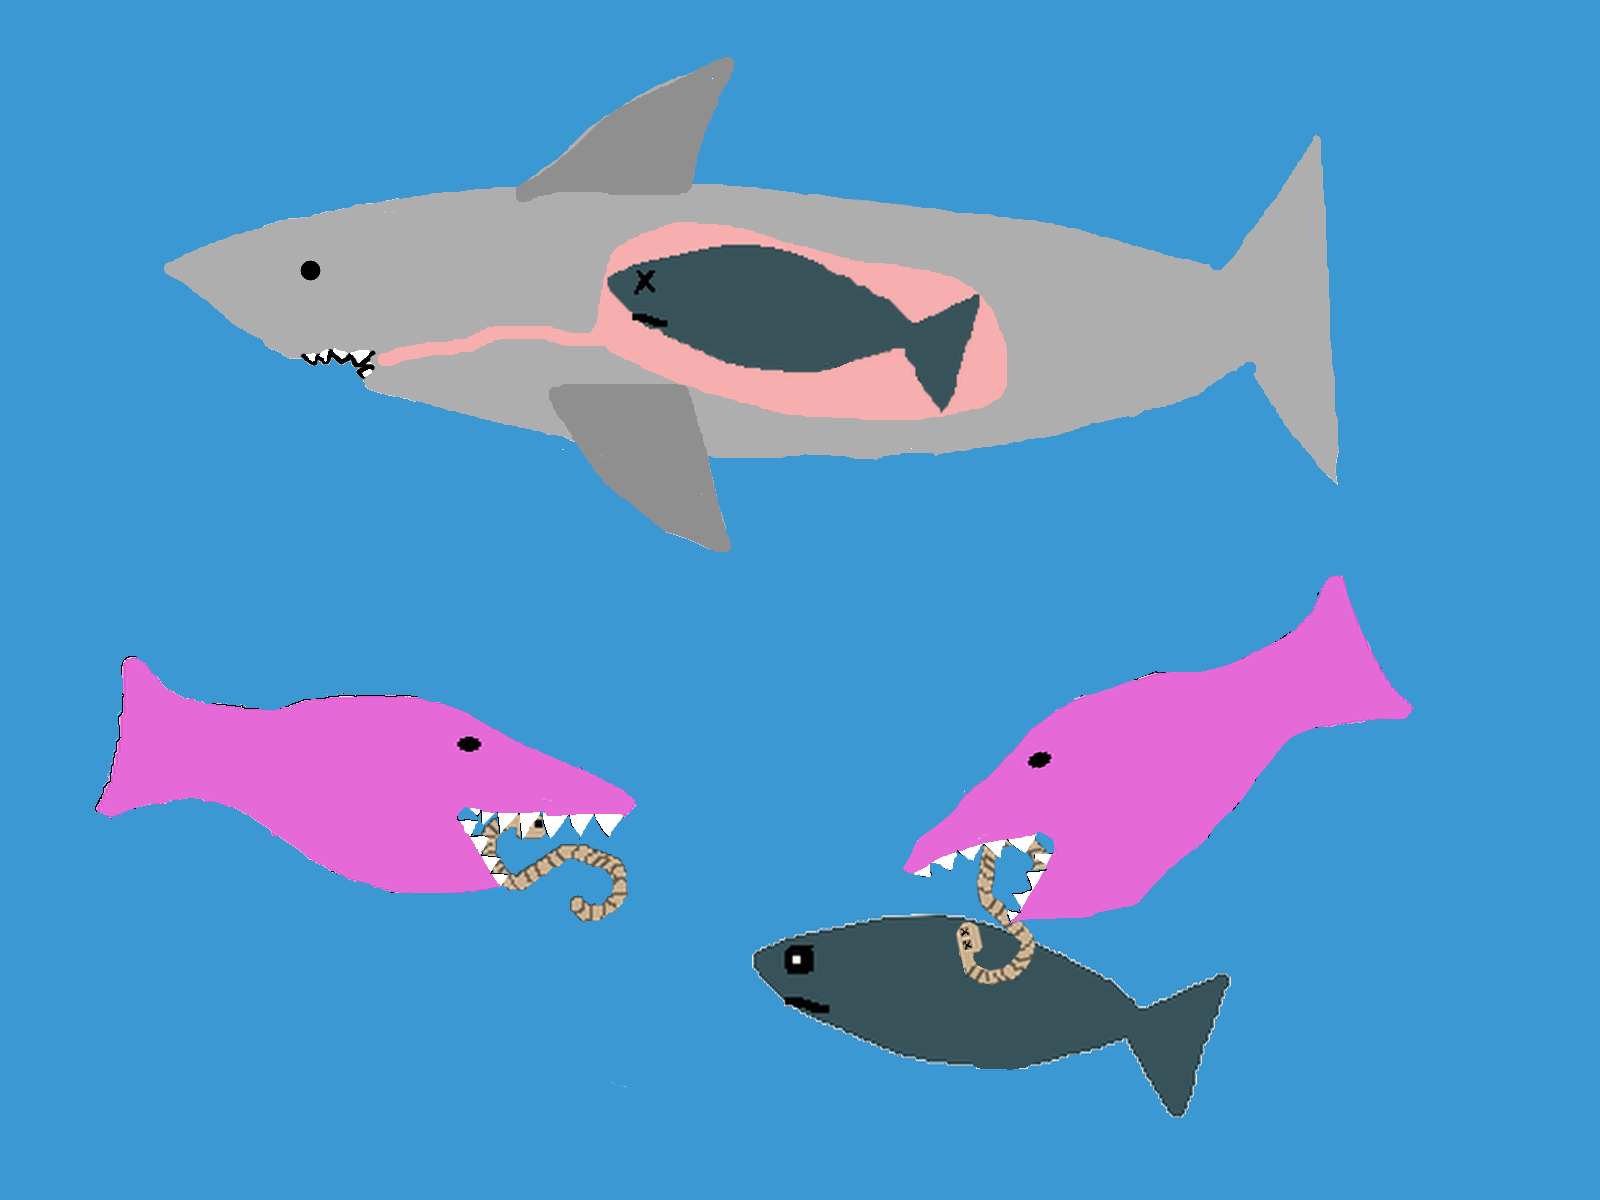
\includegraphics[width=\textwidth]{../figures/Null.png}
\end{subfigure}
\begin{subfigure}{.45\textwidth}
\caption{refuge\label{subfig:modelsb}}
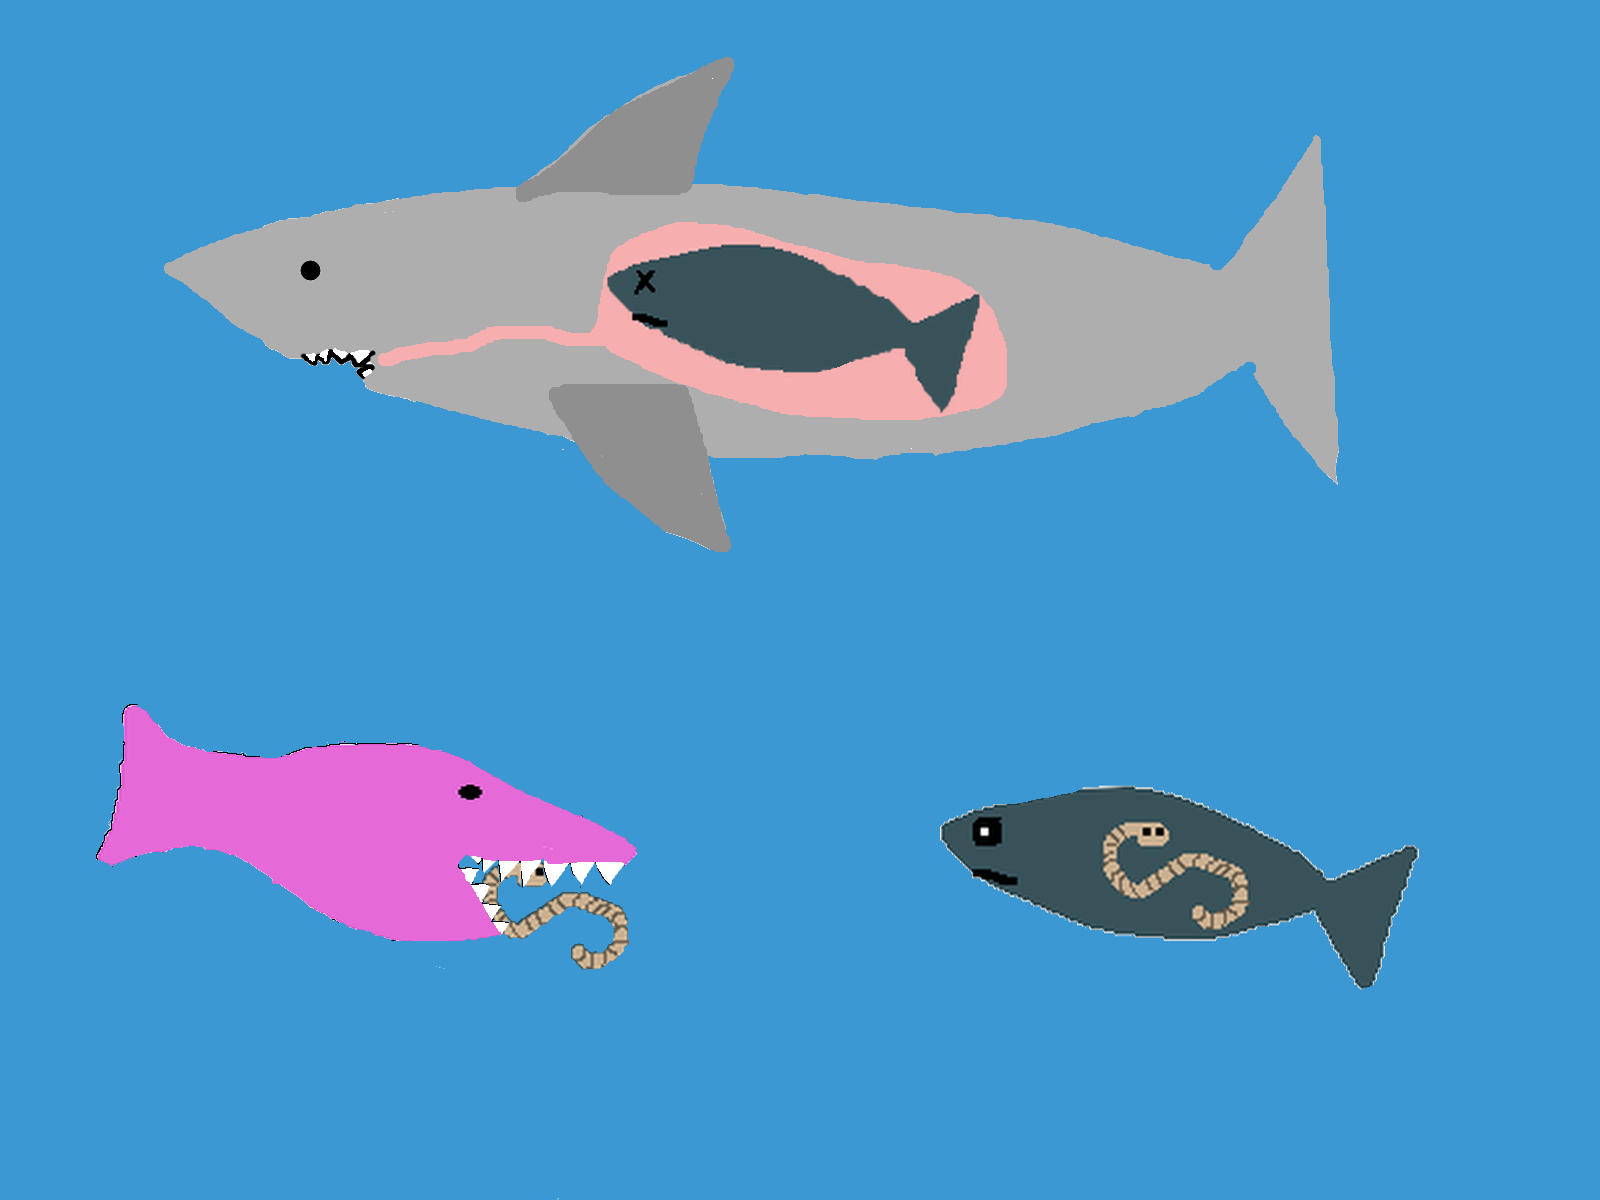
\includegraphics[width=\textwidth]{../figures/Null+Ref.png}
\end{subfigure}

\begin{subfigure}{.45\textwidth}
\caption{concomittant\label{subfig:modelsc}}
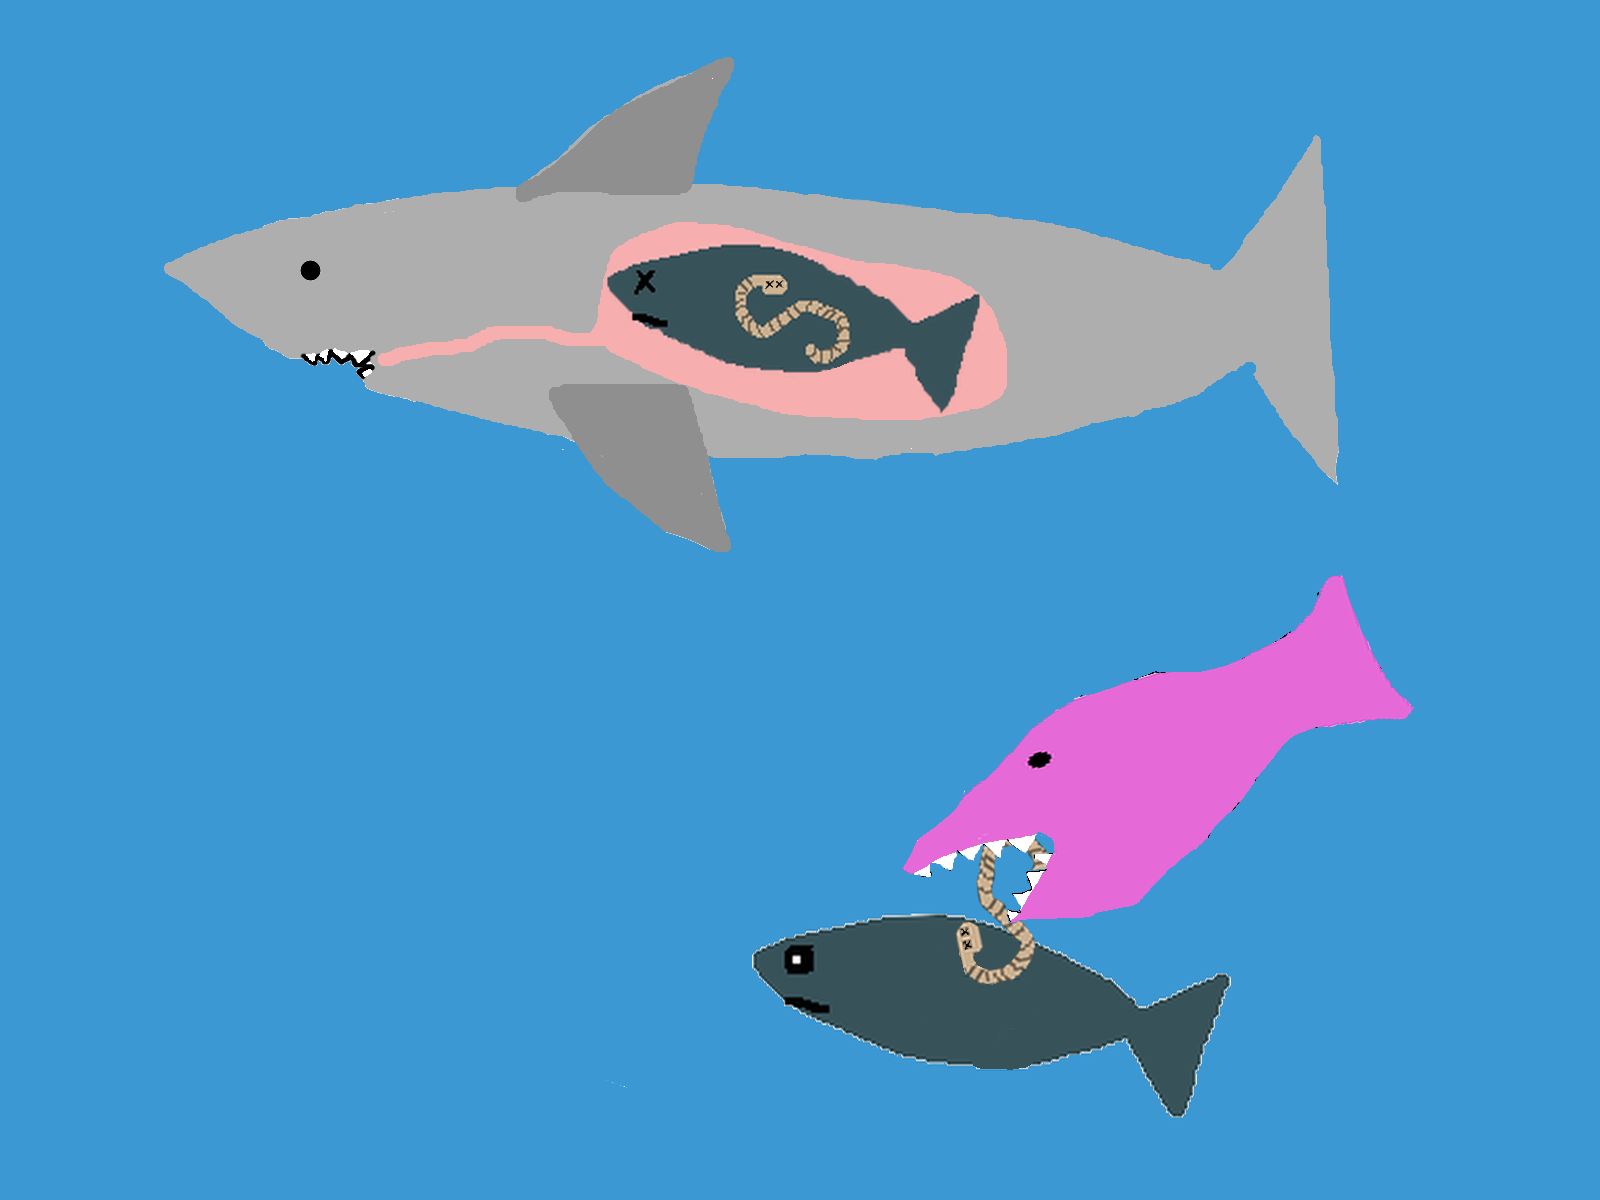
\includegraphics[width=\textwidth]{../figures/Null+Con.png}
\end{subfigure}
\begin{subfigure}{.45\textwidth}
\caption{refuge with concomittant\label{subfig:modelsd}}
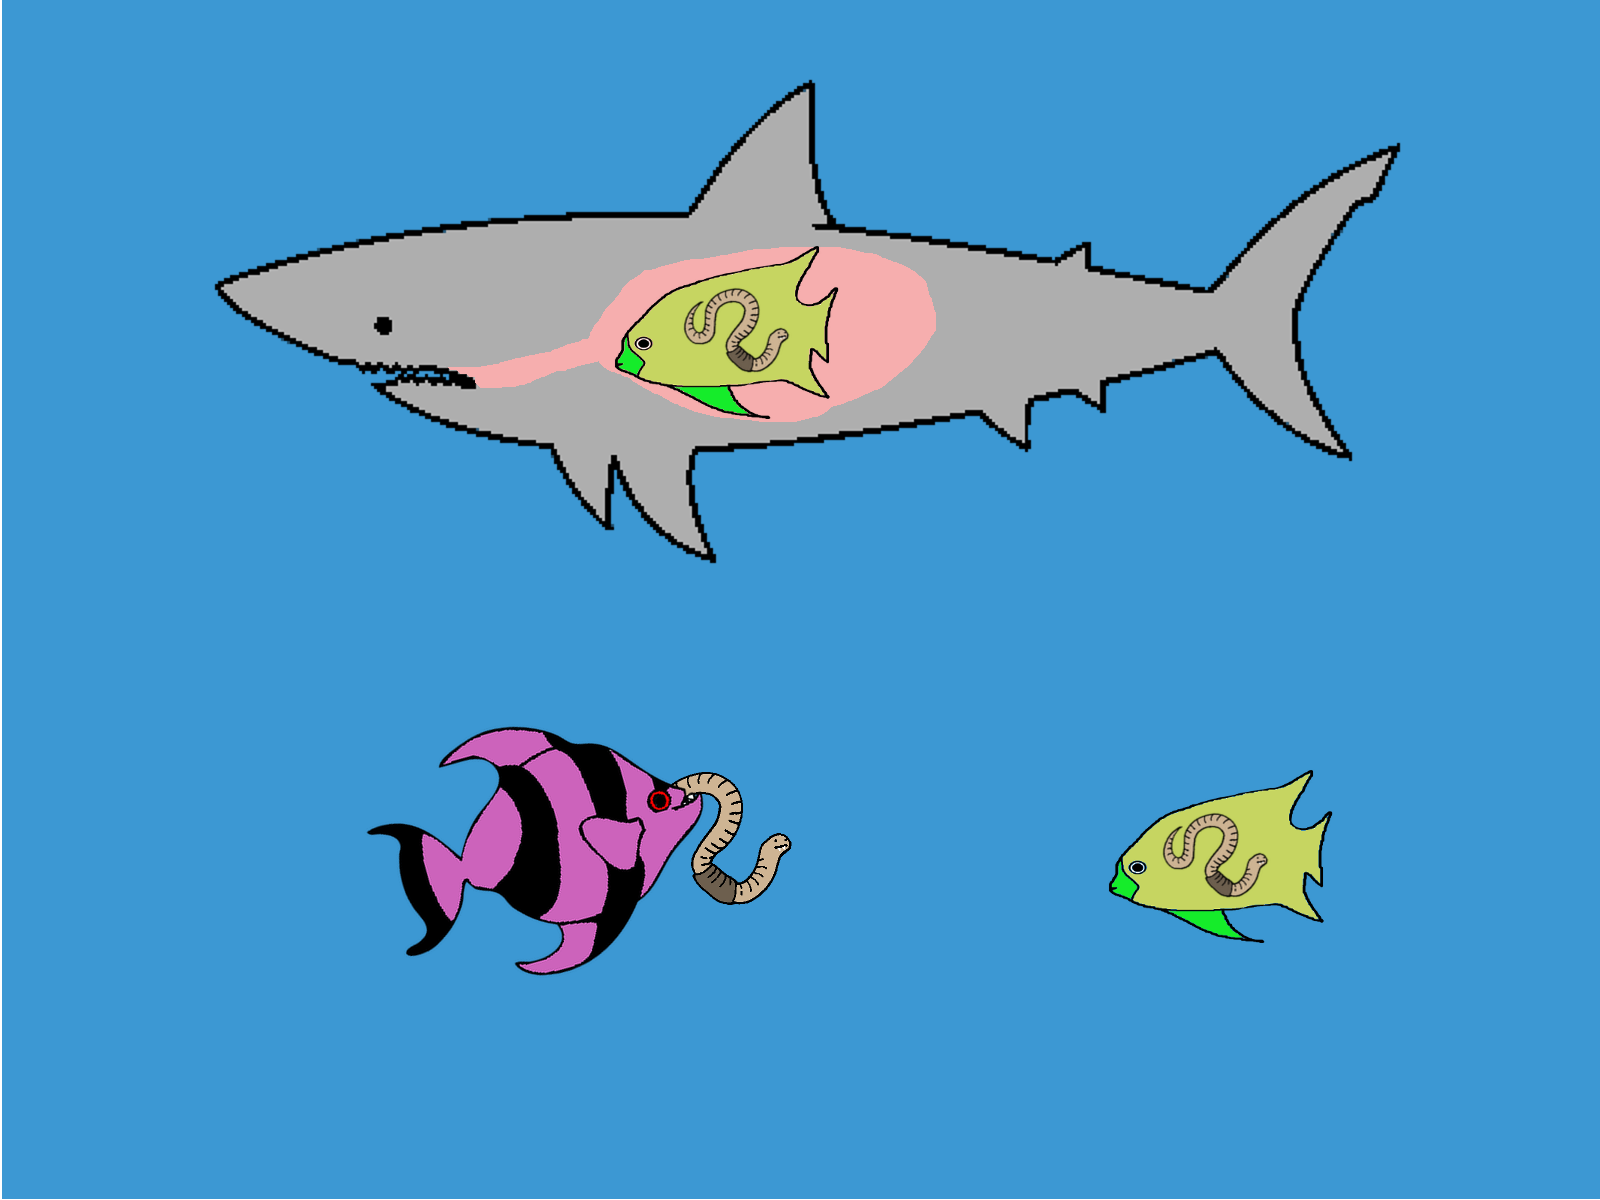
\includegraphics[width=\textwidth]{../figures/Con+Ref.png}
\end{subfigure}
\caption{This cartoon illustrates the differences between the four different versions of ATN dynamics that were tested.  \label{fig:cartoons}}
\end{figure}

In the first (null) model (figure \ref{subfig:modelsa}) parasites are vulnerable to their predators while both inside and outside their hosts and they are not susecptible to concomittant predation.  In the null model, the only things that change when a species becomes a parasite are it's body size and metabolic rate.  In the second model, (figure \ref{subfig:modelsb})  we introduce a parameter, $\phi_i$, to the null model that controls the fraction of parasitic biomass outside of a host at any given time.  A parasite is protected from predation while inside its host.  However, the parasite is also not susceptible to concomittant predation.  This represents the situation in which parasites are most protected.  The third model (figure \ref{subfig:modelsc}) modifies the null model by making parasites within their hosts susceptible to concomittant predation (see figure \ref{fig:concDiagram}).  Note that in this model we don't distinguish where a parasite is; the entire popluation is susceptible to both concomittant and normal predation.  The model in \ref{subfig:modelsc} represents the most vulnerable situation for parasites. \footnote{We could try to justify this model, but it might be better just to say that we did it this way in an attempt to separate the effects from the two modifications (since it \textit{isn't} realistic; neither \ref{subfig:modelsc} nor \ref{subfig:modelsb} are. In \ref{subfig:modelsd}, are the two modifications independent?  They do seem to be, but this is an opportunity for a neat statistical test.}  In the final model (figure \ref{subfig:modelsd}) we use the parameter $phi_i$ to determine what fraction of parasitic biomass is susceptible to concomittant predation.  The fraction of parasitic biomass that is inside a host is protected from 'normal' predation - we assume that parasites are not trophically consumed in their hosts\footnote{This is an area for potential improvement}  This was designed to be the most 'realistic' situation.

%This is a schematic for concomittant predation.
\begin{figure}
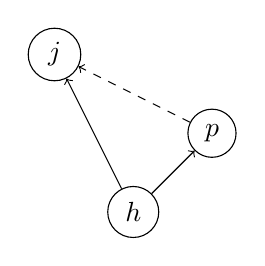
\begin{tikzpicture}
\node[draw,circle] at (0,0) (j) {$j$};
\node[draw,circle] at (1,-2) (h) {$h$};
\node[draw,circle] at (2,-1) (p) {$p$};
\draw[->] (h)--(j);
\draw[->] (h)--(p);
\draw[->,dashed] (p)--(j);
\end{tikzpicture}
\caption{This diagram illustrates concomittant predation.  The biomass of $p$ that is inside host $h$ is consumed when $h$ is eaten by its consumer, $j$. \label{fig:concDiagram}}
\end{figure}

In principle, the parameter $\phi_i$ can vary for each species for the second and fourth models (figures \ref{subfig:modelsb} and \ref{subfig:modelsd}).  Since this was not a focus of the study\footnote{though adding sensitivity to this could be in the future of this study} we used a constant fraction for all parasites and set it equal to 1 for free-livers:

\begin{equation}
\phi_i = 
\left\{
\begin{array}{c c c}
\phi & \text{if} & i:\text{ parasite}\\
1 & \text{if} & i:\text{ free-liver}\\
\end{array}\right.\label{eq:phi}
\end{equation}

The introduction of $\phi_i$ required significant changes to the ATN model (equations \eqref{eq:atn0} and \eqref{eq:fr0}):


\begin{subequations}\label{eq:atn1}
\begin{align}
\frac{dB_{b}}{dt} &= r_bB_b\left(1-\frac{\sum_{k\in\text{basal}}B_k}{K}\right) - \sum_k\phi_kB_kx_k\frac{y_{bk}F_{bk}^\text{(troph)}}{e_{bk}} - \sum_k(1-\phi_k)B_kx_k\frac{y_{bk}F^\text{(para)}_{bk}}{e_{bk}}\label{subeq:basal1} \\ 
\frac{dB_{c}}{dt} &= -x_cB_c + \phi_cx_cB_c\sum_ky_{kc}F^\text{(troph)}_{kc} + (1-\phi_c)x_cB_c\sum_ky_{kc}F^\text{(para)}_{kc} \label{subeq:con1}\\ 
& - \sum_k \phi_kx_kB_k\frac{y_{ck}F^\text{(troph)}_{ck}}{e_{ck}} - \sum_k (1-\phi_k)x_kB_k\frac{y_{ck}F^\text{(para)}_{ck}}{e_{ck}}\nonumber
\end{align}
\end{subequations}

Where the new functional responses are given by 

\begin{subequations}\label{eq:fr1}
\begin{align}F_{ij}^\text{(troph)} &= \frac{\omega_{ij}^{(troph)}(\phi_iB_i)^{1+h}}{B_0^{1+h} + \sum_k\omega^\text{(troph)}_{kj}(\phi_kB_k)^{1+h}} \label{subeq:fr1troph}\\
F_{ij}^\text{(para)} &= \frac{\omega_{ij}^{(para)}(\phi_iB_i)^{1+h}}{B_0^{1+h} + \sum_k\omega^\text{(para)}_{kj}(\phi_kB_k)^{1+h}} \label{subeq:fr1para}
\end{align}
\end{subequations}

The idea is to split the functional response according to whether a link represents classic predation or parasitism.  In the case of classic predation (equation \eqref{subeq:fr1troph}), only the portion of $j$'s biomass that is outside of a host can be a classic consumer (thus the fraction $\phi_c$ ahead of $F_{kc}^\text{(troph)}$ in equation \eqref{eq:atn0}).  Conversely, only the portion of biomass that is inside a host can be a parasitic consumer (thus the fractions $1-\phi_c$ and $1-\phi_k$ in equations \eqref{subeq:con1} and \eqref{subeq:basal1}).  Finally, a consumer (parasitic or classic) will only consume and search for the portion of biomass that is outside of hosts (Thus the $\phi_j$ and $\phi_k$ in the numerator and denominator, respectively, of equation \eqref{subeq:fr1troph}.  Thus, the preference for a particular species is now determined by $\omega_{ij}^\text{(troph)}$ in $F_{ij}^\text{(troph)}$ and $\omega_{ij}^\text{(para)}$ in $F_{ij}^\text{(para)}$.  These new preferences take into account the fact that a parasite does not have to divide its foraging time as a free-liver among its hosts.  By the same token, the parasite doesn't have to divide its 'foraging' time among its free-living (i.e. trophic) prey items when within a host.

The second addition is concomittant predation on parasites.  In models with concomittant predation (figures \ref{subfig:modelsc} and \ref{subfig:modelsd}), this is included as an additional term subtracted at the end of the consumer's equation, \eqref{subeq:con0} or \eqref{subeq:con1}.  Note that this means we don't allow biomass accumulation from concomittant consumption \textit{of} parasites in hosts.  The term can be compactly expressed as 
\begin{equation}
C_p = \sum_ha_{ph}c_h \label{cp1}
\end{equation}
where $a_{ph}$ is the amount of biomass of parasite $p$ per unit of biomass of host $h$, and $T_h$ is the total trophic consumption (total rate of biomass loss due to predation by classic consumers) of host $h$.  We define $a_{ph}$ as the relative biomass accumulation from parasitism of host $h$, relative to the total biomass accumulation to the parasite from all hosts.  So the equations are 
\begin{equation}
a_{ph} = \frac{(1-\phi_p)B_p}{B_h}\frac{y_{hp}F^\text{(para)}_{hp}}{\sum_{k}y_{kp}F^\text{(para)}_{kp}} \label{eq:aph1}
\end{equation}
when we separate the trophic and parasitic links of parasites (figure \ref{subfig:modelsd}), and
\begin{equation}
a_{ph} = \frac{B_p}{B_h}\frac{y_{hp}F_{hp}}{\sum_{k}y_{kp}F_{kp}} \label{eq:aph0}
\end{equation}
when we treat all links to parasites as parasitic (figure \ref{subfig:modelsc}).  Finally,
\begin{equation}
T_h = \sum_kx_kB_k\frac{F^\text{(troph)}_{kh}y_{kh}}{e_{kh}} \label{eq:Th1}
\end{equation}
when we separate the trophic and parasitic links of parasites (figure \ref{subfig:modelsd}), and
\begin{equation}
T_h = \sum_kx_kB_k\frac{F_{kh}y_{kh}}{e_{kh}} \label{eq:Th0}
\end{equation}
when we treat all links to parasites as parasitic (figure \ref{subfig:modelsc}).  To summarize,
\begin{equation}
C_p = \sum_h \left(\frac{(1-\phi_p)B_p}{B_h}\frac{y_{hp}F^\text{(para)}_{hp}}{\sum_{k}y_{kp}F^\text{(para)}_{kp}}\left[\sum_kx_kB_k\frac{F^\text{(troph)}_{kh}y_{kh}}{e_{kh}}\right] \right) \label{eq:cp2}
\end{equation}
when we split trophic and parasitic links (\ref{subfig:modelsd}) and
\begin{equation}
C_p = \sum_h \left(\frac{B_p}{B_h}\frac{y_{hp}F_{hp}}{\sum_{k}y_{kp}F_{kp}}\left[\sum_kx_kB_k\frac{F_{kh}y_{kh}}{e_{kh}}\right] \right) \label{cp2}
\end{equation}

We ran each model with each combination of body sizes with 11 different fractions of consumers as parasites with each web, for a total of $4\times4\times11\times 100 =17600$ simulations. 

\begin{table}
\begin{tabularx}{\textwidth}{|l|X|l|}
\hline
\multicolumn{3}{|X|}{Allometric Parameters}\\
\hline
Parameter&Description&Value\\
\hline
$a_x^{(inv)}$&Scaling constant for metabolic rate of invertebrate consumers & $0.314$\\
$z$&Consumer-resource body size ratio&variable, $n=4$\\
\hline
\hline
\multicolumn{3}{|X|}{Functional Response Parameters}\\
\hline
Parameter&Description&Value\\
\hline
$b_0$&Half-saturation density&$0.5$\\
$h$&Hill coefficient modifier& $0.2$\\
$\omega_{ij}$&Preference of $i$ for $j$&$1$ or $0$\\
\hline
\hline
\multicolumn{3}{|X|}{ATN Parameters}\\
\hline
Parameter&Description&Value\\
\hline
$r_i$&Intrinsic growth of producer $i$&$\mathcal{N}(1,0.1)$\\
$K$&Community carrying capacity of producers &5\\
$x_i$&Metabolic rate of consumer $i$&$a_x m_i^{-0.25}$\\
$y_i$&Maximum rate of assimilation relative to metabolic rate for invertebrate consumers & 8\\
$e_{ij}^{(carn.)}$&Assimilation efficiency of $j$ by $i$ for a consumer $j$ (carnivory) & 0.85\\
$e_{ij}^{(herb.)}$&Assimilation efficiency of $j$ by $i$ for a producer $j$ (herbivory) & 0.45\\
\hline
\hline
\multicolumn{3}{|X|}{Food Web Parameters}\\
\hline
Parameter&Description&Value\\
\hline
$s$&Species richness&40\\
$c$&Connectance & 0.15\\
\hline
\hline
\multicolumn{3}{|X|}{Independent Variables}\\
\hline
Parameter & Values or Description & Replicates\\
$z_\text{free}$&$z=10,100$&2\\
$z_\text{para}$&$z=.001,.0001$&2\\
$i_p$&concomittant loss (y/n)&2\\
$\phi$&Differentiate parasitic biomasses inside and outside hosts (y/n)&2\\
$f_{par}$&Fraction of consumers as parasites (evenly spaced between 0 and .5)&11\\
\hline
\end{tabularx}
\caption{Values of all constants used in the models.  \label{tab:param}}
\end{table}

\bibliography{../Bib_green}{}
\bibliographystyle{apalike}
\end{document}  
